\section{Dataset}\label{dataset}

To optimise the construction of predictive algorithms, the input data is divided into several datasets with different roles. Typically, a specific partition of the data into three datasets is used: \textbf{training}, \textbf{validation} and \textbf{test set}.


\begin{defi}[Training set]
    The \textbf{training set} is a set of examples used during the learning process to determine (or learn) optimal combinations of parameters.
\end{defi}

In practice, it is on the data of the training set that the chosen optimisation method is performed, thus updating the values of the parameters or hyper-parameters.

\begin{defi}[Validation set]
    The \textbf{validation set} is an independent data set used to evaluate the model trained on the training set.
\end{defi}
The evaluation (or \textit{validation}) of the model on the validation set leads to deciding which are the best values for the parameters (or hyper-parameters) based on the performance on the validation set. In the case of the elaboration set, an early-stopper is used, which chooses as the best model the one with the lowest error just before overfitting occurs.

\begin{defi}[Test set]
    A \textbf{test set} is an independent set of data from the training set used only to evaluate the performance of the model.
\end{defi}

\newpage

That is, the test set is used to evaluate on a third independent data set the chosen model based on the performance on the validation set. Performance characteristics such as accuracy, sensitivity, specificity... are thus obtained. This dataset is important because it allows the model's performance to be evaluated on a third dataset independent of the previous ones, avoiding the risk of overfitting: if a model trained on the test set also fits the test set, minimal overfitting has occurred.

The problem of \textbf{overfitting} has been mentioned several times, so the definition is given.

\begin{defi}[Overfitting]
    Overfitting is the generation of a model (or analysis) that corresponds too closely to a particular data set and may therefore fail to predict future observations reliably.
\end{defi}

Overfitting may occur, for example, by including too many adjustable parameters or by using an approach that is too complicated, as shown in figure \ref{overfittigComplex}. Clearly, when comparing different types of models, the complexity must take into account the influence of each parameter on the output \footnote{ Note that the opposite problem can be encountered by using an approach that is too simple: underfitting. For example, trying to approximate a sample with a parabolic trend with a linear regression}.

\begin{figure}[htbp]
    \centering
    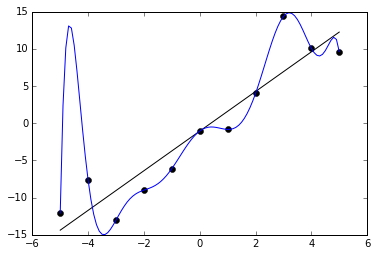
\includegraphics[width=0.6\textwidth]{images/Machine learning/Overfitted_Data.png}
    \caption{Example of overfitting. Data (approximately linear) are approximated by a linear function and a polynomial function. Although the polynomial function provides an almost perfect fit, the linear function can be expected to generalise the data better. \cite{wiki:overfitting}}
    \label{overfittigComplex}
\end{figure}

\newpage

Overfitting is particularly likely in cases where learning has been performed for too long or where there is little data for learning, causing the model to fit very specific random features of the training data that have no causal relationship with the output. In this case of overfitting, the performance on the training set continues to increase while the performance on the validation set deteriorates, as shown in figure \ref{overfittingError}.



\begin{figure}[htbp]
    \centering
    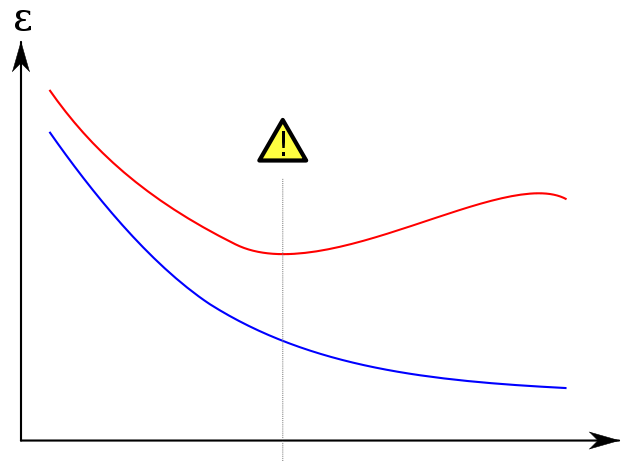
\includegraphics[width=0.6\textwidth]{images/Machine learning/Overfitting error.png}
    \caption{Overfitting in supervised learning. The training error (error on training set) is shown in blue, the validation error (error on validation set) in red, both as a function of the number of training cycles. \cite{wiki:overfitting}}
    \label{overfittingError}
\end{figure}


\subsection{Loss function}
So far, the problem that interests the paper has been outlined: looking for a function $f$ to predict the output $Y$ from the values of the input $X$. This requires a loss function, $L(Y, f (X))$ to penalise prediction errors.

\begin{defi}[Loss function]
    A \textbf{loss function} is a function in the form $\mathcal{L}(y_{\text{true}},y_{ \text{guess}})$ that defines the loss incurred (or the error committed) by predicting the value $y_{\text{guess}}$ when the true value is $y_{\text{true}}$, thus providing an evaluation of the model's predictive capabilities.
\end{defi}

This will be the function to be minimised by an optimisation algorithm for fitting the hyperparameters of the Gaussian process. Obviously, the choice of loss function depends on the context.

%\section{Mean squared error}
%Per gli scopi dell'elaborato, si farà uso del \textit{mean squared error}.

%\begin{defi}[Mean squared error]
%Il \textbf{mean squared error} (o \textit{MSE}) è una \textit{loss function} definita come:
%\[
%\frac{1}{n}\sum^{n}_{i=1}(Y_i-f(X_i))^2,
%\]
%dove su $n$ dati raccolti, $Y_i$ sono gli output reali, $f(X_i)$ sono gli output predetti a partire da $X_i$.
%Poiché deriva dal quadrato della distanza euclidea, è sempre un valore positivo che diminuisce man mano che l'errore si avvicina a zero.
%\end{defi}
%Verrà usato non come loss function, ma per monitorare l'andamento del training.


%\section{Coefficiente di determinazione}
%Il coefficiente di determinazione fornisce una misura della bontà di adattamento di un modello, cioè quanto le previsioni di regressione approssimano i punti dei dati reali. Varia tra 0 e 1\footnote{Si possono apportare modifiche al coefficiente per fargli assumere anche altri valori, ma non vengono applicate nell'elaborato}, un $R^2$ di 1 indica che le previsioni di regressione si adattano perfettamente ai dati.

%Poichè il coefficiente di determinazione varia in un intervallo unitario, può essere più (intuitivamente) informativo di altre misure di errore (come il mean absolute error o il mean squared error) poiché tendono ad assumere valori su intervalli arbitrari oppure ad esprimere una percentuale.

%\begin{defi}[Coefficiente di determinazione]
%Date $y_i$ le osservazioni, $\overline{y}$ la media delle osservazioni, $\hat{y}_i$ i dati predetti dal modello:
%\[
%R^2 = 1-\frac{\sum_{i=1}^{n}(y_i-\hat{y}_i)}{\sum_{%i=1}^{n}(y_i-\overline{y})}
%\]
%\end{defi}
%Si noti che questo coefficiente non indica se:
%\begin{itemize}
%    \item una variabile sia statisticamente %significativa;
%    \item è stata usata la regressione corretta;
%    \item è stato scelto l'insieme più appropriato %di variabili indipendenti;
%    \item ci sono abbastanza dati per trarre una %conclusione solida.
%\end{itemize}

%Si noti inoltre che $R^2$ è una versione riscalata del mean squared error più facile da interpretare in quanto non dipende dalla scala dei dati.